\documentclass[aspectratio=169]{beamer}

\usepackage{graphicx}
\usepackage{color}
\usepackage{amsmath}
\usepackage{pgffor}
\usepackage{listings}

\definecolor{darkred}{rgb}{0.8,0,0}
\definecolor{darkgreen}{rgb}{0,0.8,0}
\definecolor{lightgray}{rgb}{0.9,0.9,0.9}

\mode<presentation> {\usetheme{CambridgeUS} \usecolortheme{beaver}}
\setbeamercolor*{item}{fg=red}
\setbeamercolor{block title}{bg=lightgray,fg=darkred}
\setbeamertemplate{navigation symbols}{}

\title[Stability and Control Synthesis via Convex Optimization]{Stability Analysis and Optimal Control Synthesis via Convex Optimization}
% control synthesis via convex optimization

\author{Tobia Marcucci}
\institute{\textit{tobiam@mit.edu}}
\date{July 30, 2020}

\begin{document}

\begin{frame}
\titlepage
\end{frame}

\section{Introduction}
\begin{frame}
\huge
\centering
{\color{darkred} Introduction}
\end{frame}

\begin{frame}{Quick recap}
The main topic so far:
\begin{align*}
v(x_0) := \min_{u, x} \ &\int_0^\infty l(x(t), u(t)) dt \\
\text{subject to} \ & x(0) = x_0 \\
& \dot x(t) = f(x(t), u(t)), &&  \text{for all }t \in [0, \infty) \\
& u(t) \in U, &&  \text{for all }t \in [0, \infty)
\end{align*}
\begin{itemize}
\item
Pontryagin's minimum principle (\textbf{analytical}):
\begin{itemize}
\item
necessary conditions for optimality as a two-point boundary value problem
\item
closed-form solution only in very few special cases
\end{itemize}
\item
Numerical optimization (\textbf{numerical}):
\begin{itemize}
\item
in general, a nonconvex program
\item
for linear systems, convex objective and constraints, a convex program
\end{itemize}
\end{itemize}
\end{frame}

\begin{frame}{Working with time is not the only option}
A classical example: \textbf{Lyapunov stability} is much easier in state space than in time
\begin{columns}
\column{.8\textwidth}
\begin{itemize}
\item
An ODE such as
$$
\ddot \theta(t) + \dot \theta(t) + \sin(\theta(t)) = 0
$$
does not have closed-form solution $\theta(t)$
\item
Asymptotic stability ($\lim_{t \rightarrow \infty} \theta(t) = 0$) can be easily proved by showing that the energy
$$
v(\theta, \dot \theta) := \frac{1}{2} \dot \theta^2 - \cos(\theta)
$$
converges to zero
\end{itemize}
\column{.2\textwidth}
\begin{figure}[h]
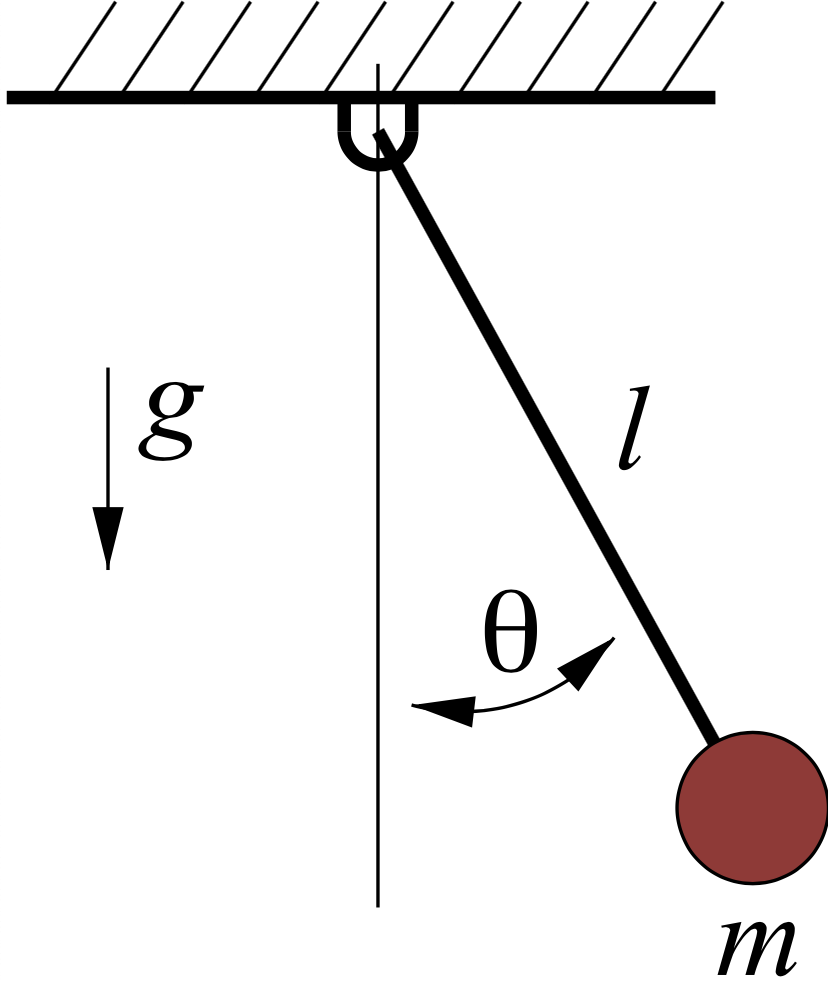
\includegraphics[width=\columnwidth]{figures/simple_pend.png}
\end{figure}
\end{columns}
\begin{block}{Lyapunov theorem}
``$\dot x = f(x)$ is stable if there exists $v(x) \geq 0$ such that $\dot v(x) = \frac{\partial v}{\partial x} (x) f(x) \leq 0$''
\end{block}
\end{frame}

\begin{frame}{Dynamic programming}
The state-space approach to optimal control is called \textbf{Dynamic Programming} (DP), and at its core we have the \textbf{Hamilton-Jacobi-Bellman} (HJB) equation
\begin{align*}
\min_{u \in U} \left\{ l(x, u) + \frac{\partial v}{\partial x} (x) f(x, u) \right\} = 0, \quad \text{for all } x
\end{align*}
\begin{itemize}
\item
Recall that $v(x_0)$ is the minimum of the optimal control problem for $x(0) = x_0$
\end{itemize}
\textbf{DP $:$ optimal control $=$ Lyapunov theorem $:$ stability}? Not quite...
\begin{itemize}
\item
In time, optimal control has similar issues to stability (hard ODEs)
\item
In state space:
\begin{itemize}
\item
HJB is a nasty {\color{darkred} nonlinear} partial differential {\color{darkred} equation}
\item
Lyapunov conditions ($v(x) \succeq 0$, $\dot v(x) \preceq 0$) are nice {\color{darkgreen} linear} differential {\color{darkgreen} inequalities}
\end{itemize}
\end{itemize}
\end{frame}

\begin{frame}{Quoting the authors}
\begin{columns}
\column{.5\textwidth}
\begin{columns}
\column{.2\columnwidth}
\begin{figure}
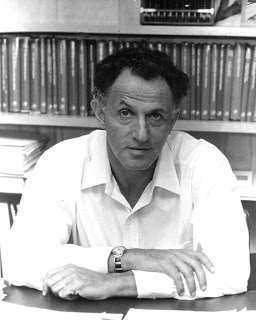
\includegraphics[width=\columnwidth]{figures/bellman.jpg}
\end{figure}
\column{.75\columnwidth}
Bellman, \\ ``Dynamic Programming'' (1957)
\end{columns}
\begin{figure}[h]
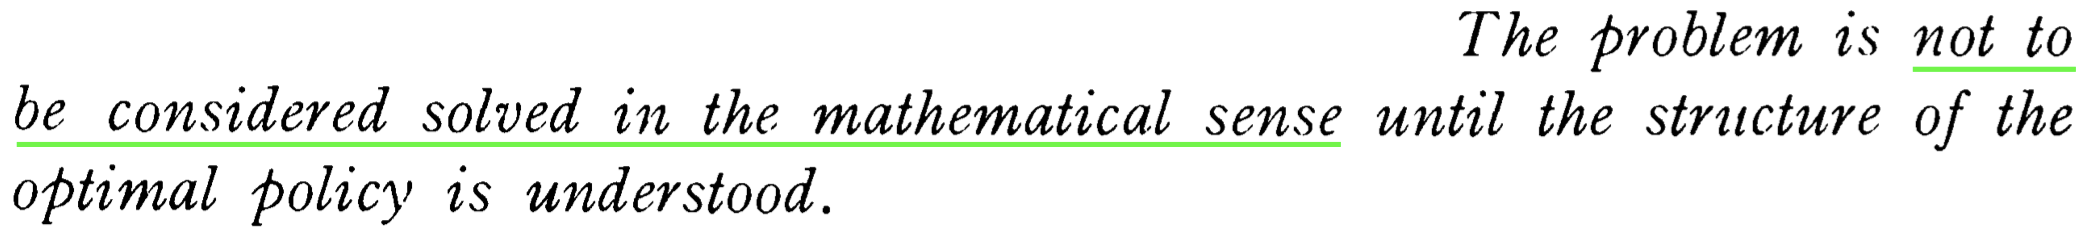
\includegraphics[width=.9\columnwidth]{figures/bellman_quote_1.png} \\
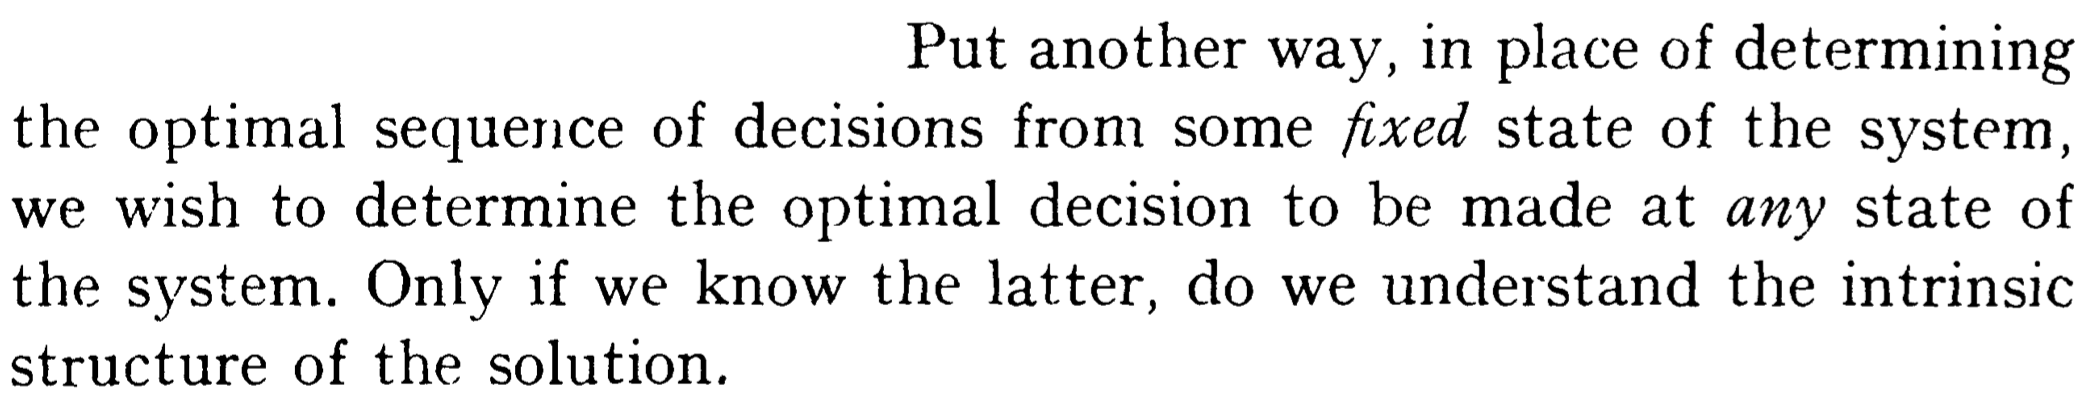
\includegraphics[width=.9\columnwidth]{figures/bellman_quote_2.png} \\
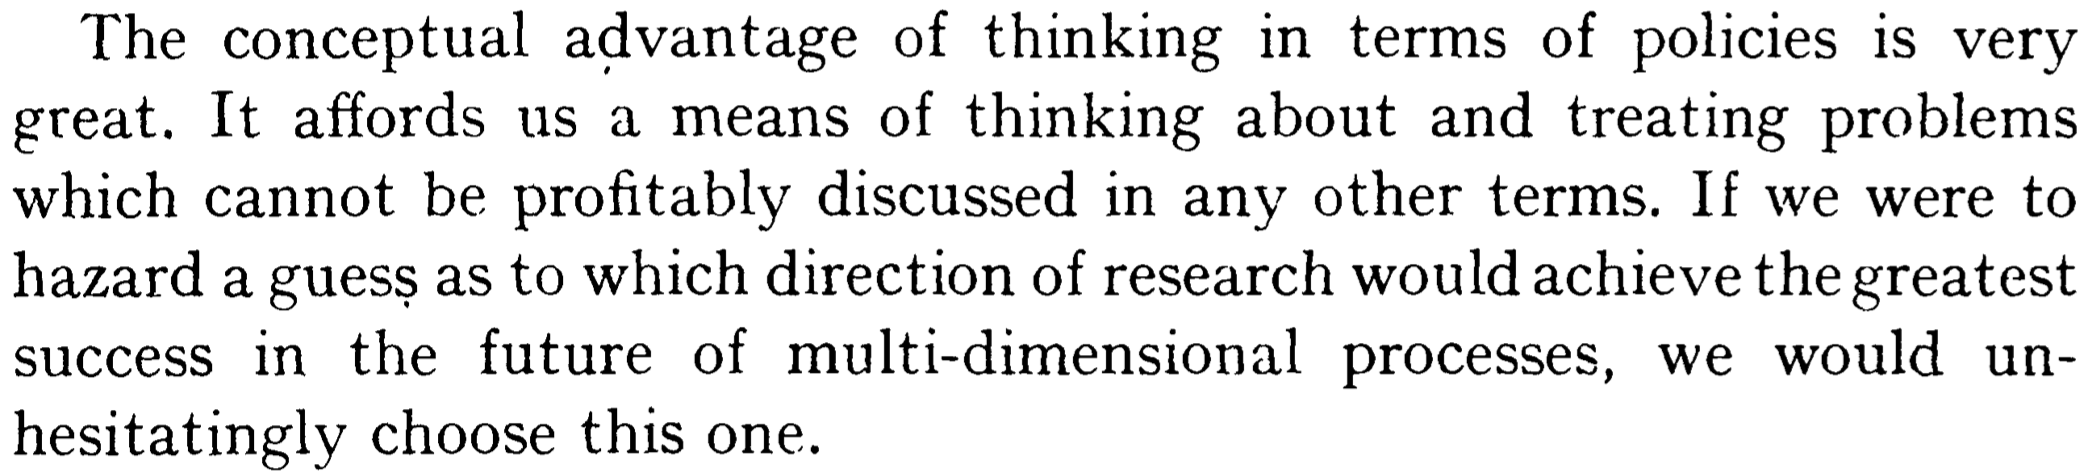
\includegraphics[width=.9\columnwidth]{figures/bellman_quote_3.png}
\end{figure}
\column{.5\textwidth}
\begin{columns}
\column{.15\columnwidth}
\begin{figure}
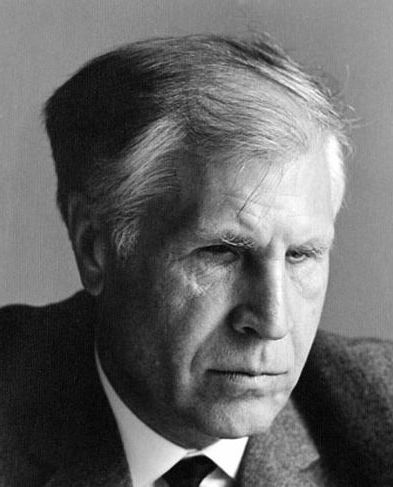
\includegraphics[width=\columnwidth]{figures/pontryagin.jpg}
\end{figure}
\column{.75\columnwidth}
Pontryagin et al., \\
``The Mathematical Theory of Optimal Processes'' (1962)
\end{columns}

\begin{figure}[h]
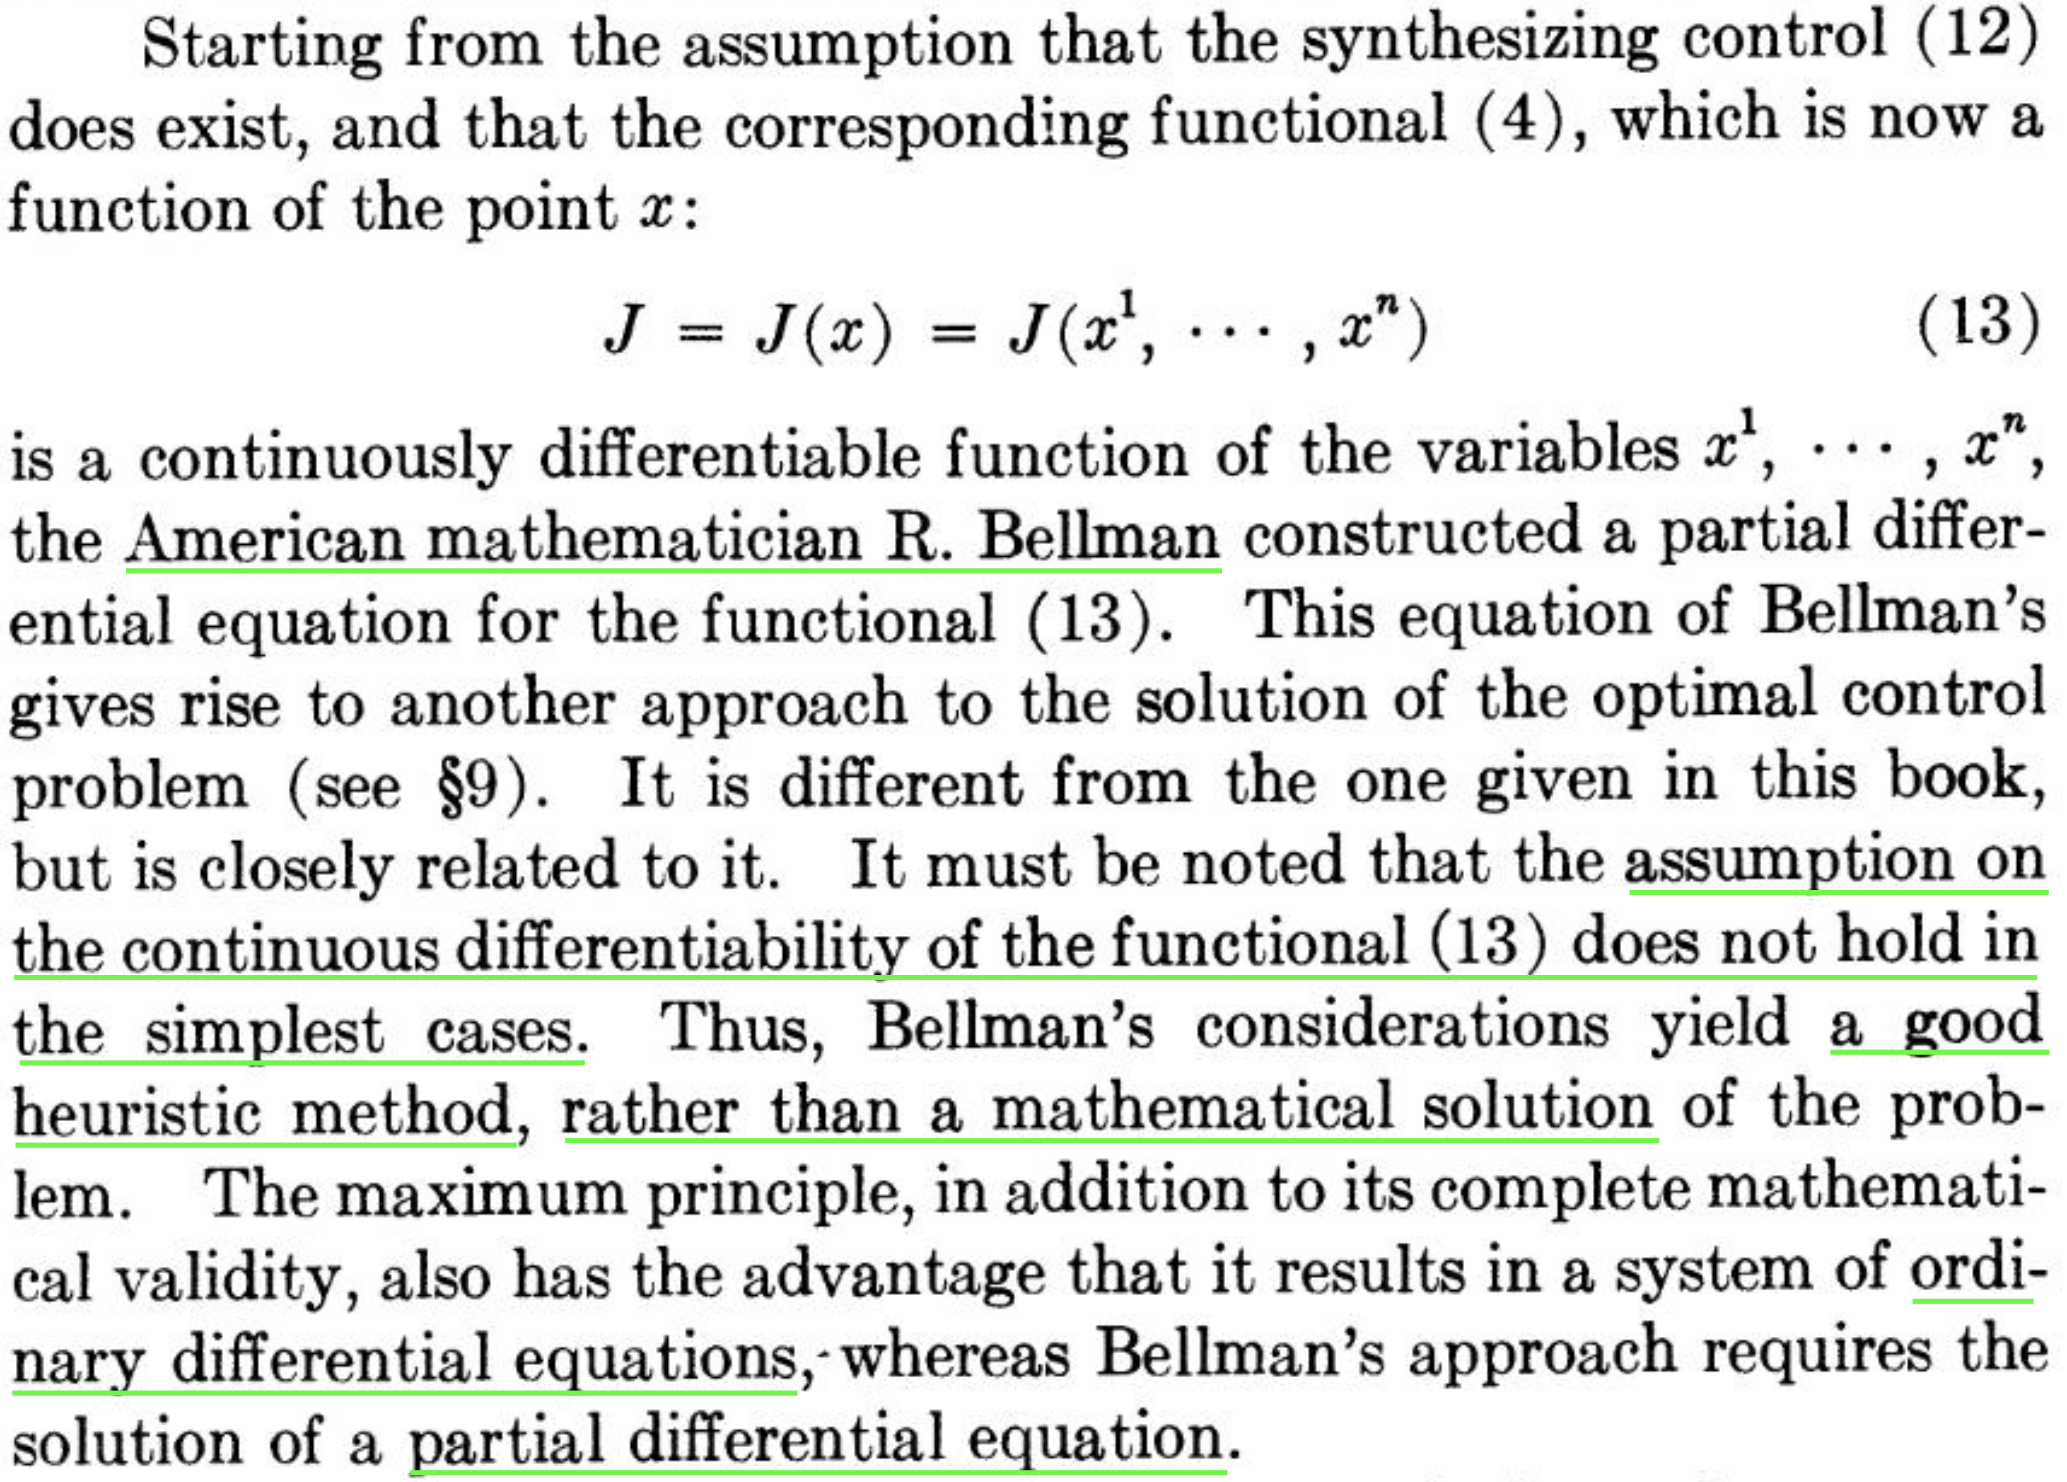
\includegraphics[width=.9\columnwidth]{figures/pontryagin_quote.png}
\end{figure}
\end{columns}
\end{frame}

\begin{frame}{Our goal today}
Use \textbf{convex optimization} to design functions in state space:
\begin{itemize}
\item
SemiDefinite Programming (SDP)
\item
Sums-of-Squares (SOS) optimization
%\item
%Pretty soon we'll restrict our class of function to polynomials
\end{itemize}

We'll focus on \textbf{two main applications}:
\begin{itemize}
\item
Design of Lyapunov functions
\begin{itemize}
\item
Not really optimal control, but of fundamental importance
\item
Convex optimization will be a game changer here
\end{itemize}
\item
Approximate dynamic programming
\begin{itemize}
\item
Convex optimization will still be pretty effective here
\end{itemize}
\end{itemize}
\end{frame}

\section{Convex-optimization background}
\begin{frame}
\huge
\centering
{\color{darkred} Convex-optimization background}
\end{frame}

\begin{frame}{Convex optimization recap}
\begin{columns}
\column{.5\textwidth}
With $f_0, \ldots, f_n$ convex functions
\begin{align*}
\min_{x} \ &f_0(x) \\
\text{subject to} \ & x(0) = x_0 \\
& f_i(x) \leq 0, &&  i = 1, \ldots, m \\
& a_i^T x = b_i, &&  i = 1, \ldots, p
\end{align*}
Fundamental property:
\begin{itemize}
\item
{\color{darkgreen}every local minimum is a global minimum}
\end{itemize}
\column{.5\textwidth}
\begin{figure}
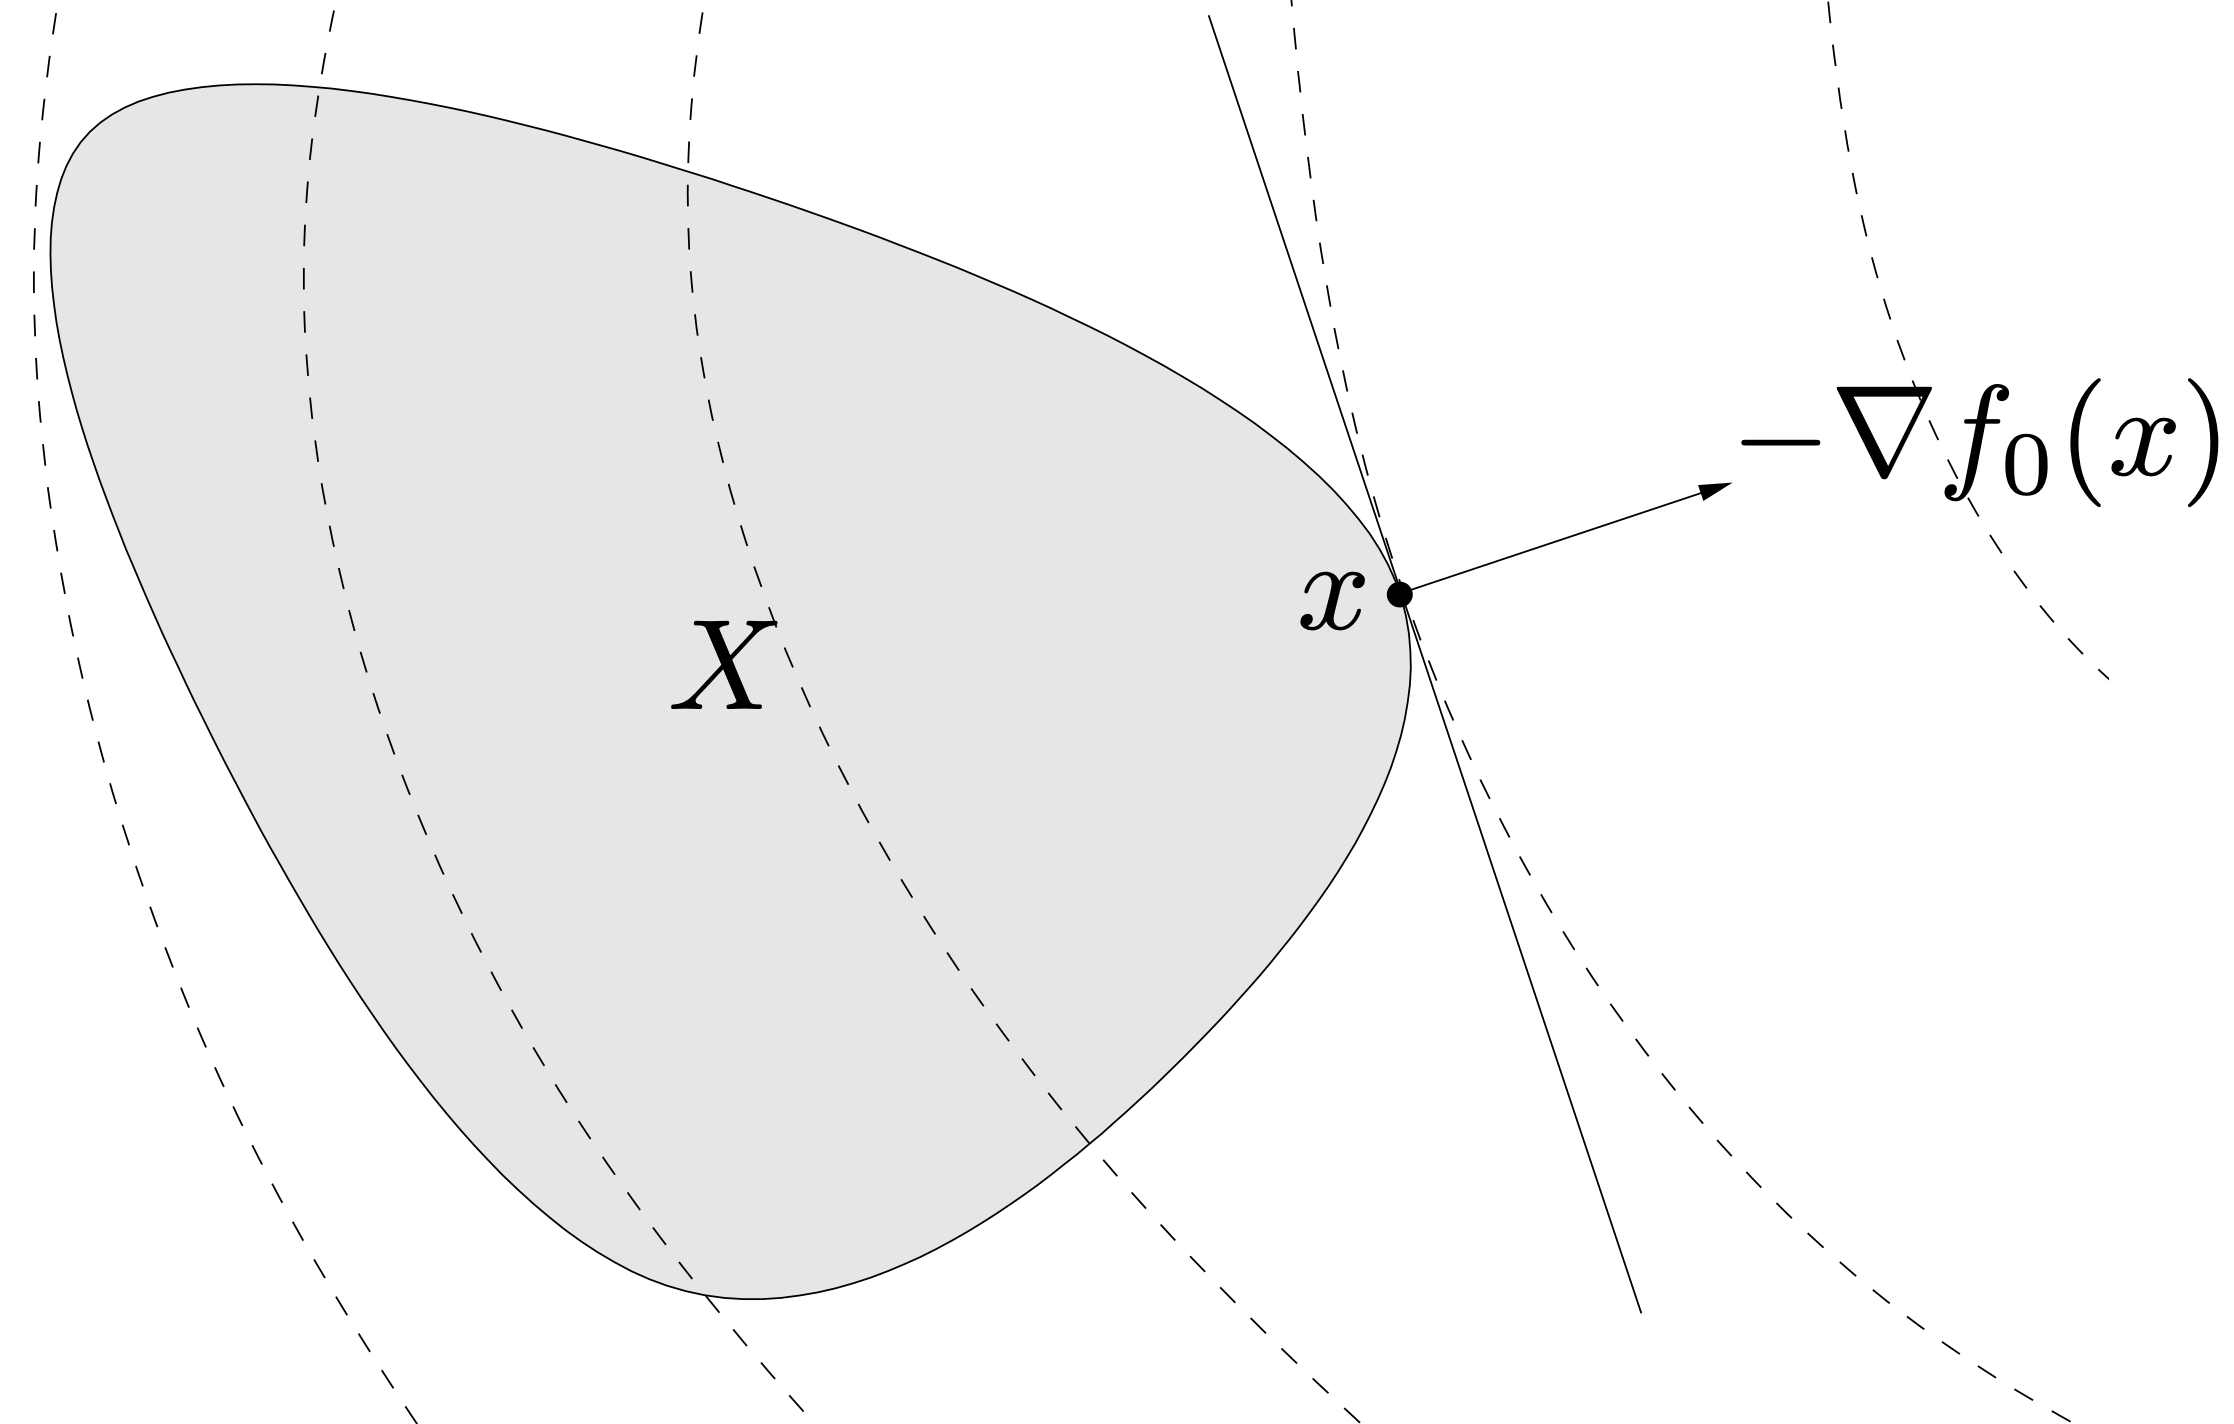
\includegraphics[width=\columnwidth]{figures/convex_opt.png}
\footnotesize Boyd, Vandenberghe - ``Convex Optimization''
\end{figure}
\end{columns}
\end{frame}

\begin{frame}{Proof of ``every local minimum is global''}
\begin{itemize}
\item
If $x^*$ is a local minimum, there exists $r > 0$ such that
$$
x^* = \arg \min_x \{ f_0(x) : x \text{\ is feasible}, \|x - x^*\| \leq r \}
$$
\item
If $x^*$ was not a global minimum, there would exist $y$ feasible such that $f_0(y) < f_0(x^*)$
\item
Necessarily, $\|y - x^*\| > r$
\item
Take a point $z$ on the line connecting $x^*$ and $y$, distant $r/2$ from $x^*$:
$$
z = x^* + \theta (y - x^*) = (1 - \theta) x^* + \theta y, \quad \theta = \frac{r}{2 \|y - x^*\|}
$$
\item
By convexity of the feasible set, $z$ is feasible
\item
By convexity of the objective,
$$
f_0(z) \leq (1 - \theta) f_0(x^*) + \theta f_0(y) < (1 - \theta) f_0(x^*) + \theta f_0(x^*) = f_0(x^*)
$$
which contradicts the local optimality of $x^*$
\end{itemize}
\end{frame}

\begin{frame}{Classes of convex optimizations}
\begin{columns}
\column{.7\textwidth}
Many classes of Convex Programs (CPs):
\begin{itemize}
\item
Linear Programs (LPs) are the easiest
\item
SemiDefinite Programming (SDP) is a broad class of CPs that can be solved efficiently (our main tool today)
\item
Some CPs outside the class of SDP can be quite hard
\end{itemize}
What do we mean by ``hard convex optimizations''? 
\begin{itemize}
\item
Interior-point methods require a function to repel a point from the boundary of the feasible set
\item
Some convex sets are very hard to describe mathematically!
\item
We'll come back to this point...
\end{itemize}
\column{.3\textwidth}
\begin{figure}
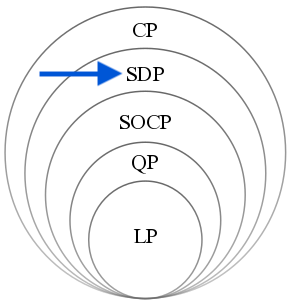
\includegraphics[width=\columnwidth]{figures/hierarchy.png}
\end{figure}
\end{columns}
\end{frame}

\begin{frame}{Definite symmetric matrices}
Equivalent statements for a symmetric $A$:
\begin{itemize}
\item
$A$ is \textbf{positive semidefinite} (denoted as $A \succeq 0$)
\item
$x^T A x \geq 0$ for all $x$
\item
The eigenvalues $\lambda_1, \ldots, \lambda_n$ of $A$ are nonnegative
\item
There exists $L$ such that $A = L^T L$
\end{itemize}
What's the \textbf{relation with convex optimization}?
\begin{itemize}
\item
let 
$$
A = \begin{bmatrix}
a_{11} & a_{12} & \cdots & a_{1n} \\
a_{12} & a_{22} & \cdots & a_{2n} \\
\vdots & \vdots & \ddots & \vdots \\
a_{1n} & a_{2n} & \cdots & a_{nn} \\
\end{bmatrix}
$$
\item
the set $\mathbb S_n^+ := \{ (a_{11},\dots, a_{nn}) : A \succeq 0 \}$ is convex
\end{itemize}
\end{frame}

\begin{frame}{Proof of ``$\mathbb S_n^+$ is convex''}
\begin{columns}
	\column{.53\textwidth}
Just use the definition:
\begin{itemize}
	\item
	assume $A_1 \succeq 0$ and $A_2 \succeq 0$
	\item
	let $A := \theta A_1 + (1- \theta) A_2$ with $\theta \in [0, 1]$
	\item
	then $x^T A x = \theta x^T A_1 x + (1- \theta) x^T A_2 x \geq 0$ for all $x$
\end{itemize}
	\column{.45\textwidth}
	\begin{figure}
		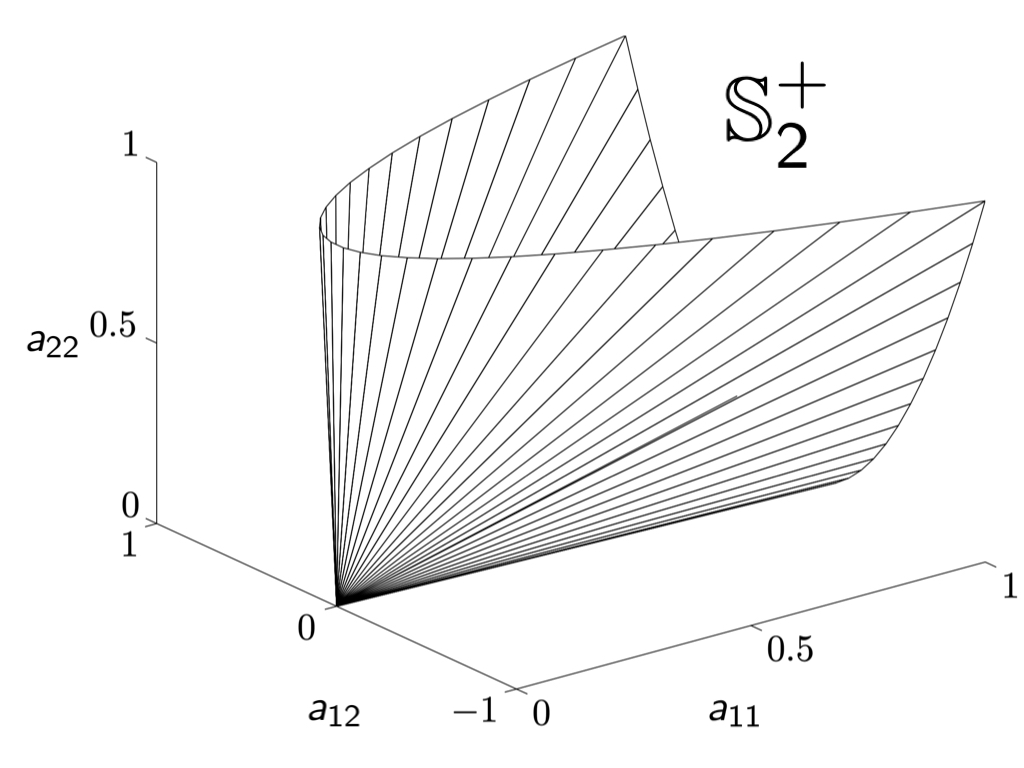
\includegraphics[width=\columnwidth]{figures/psdcone.jpeg}
		\footnotesize Boyd, Vandenberghe - ``Convex Optimization''
	\end{figure}
\end{columns}
\end{frame}

\begin{frame}{Semidefinite program in standard form}
\begin{columns}
	\column{.5\textwidth}
\begin{align*}
\min_{X} \ & \text{tr}(C X) \\
\text{subject to} \ & \text{tr}(A_i X) = b_i, &&  i = 1, \ldots, p \\
& X \succeq 0
\end{align*}
\column{.5\textwidth}
\begin{itemize}
\item
recall that, e.g., $\text{tr}(C X) = \sum_{i,j=1}^n C_{ij} X_{ij}$
\item
linear objective function (convex)
\item
$p$ linear equality constraints (convex)
\item
one semideifinite constraint (convex)
\end{itemize}
\end{columns}
\vspace{5mm}
Why is SDP efficient?
\begin{itemize}
\item
What's a nice function to repel a point $(a_{11},\dots, a_{nn})$ from the boundary of the feasible set?
\item
Interior of the feasible set is $\{ (a_{11},\dots, a_{nn}) : \lambda_1 > 0, \ldots, \lambda_n > 0 \}$
\item
Natural candidate: $$- \sum_{i=1}^n \ln (\lambda_i) = - \ln( \prod_{i=1}^n \lambda_i ) = - \ln (\det A)$$
\end{itemize}
\end{frame}

\section{Sums-of-squares optimization}
\begin{frame}
\huge
\centering
{\color{darkred} Sums-of-squares optimization}
\end{frame}

\begin{frame}{Nonlinear parameterization of the function space}
\begin{itemize}
\item
Ultimately, we want to use convex optimization to design functions $v(x) : \mathbb R^n \mapsto \mathbb R$
\item
\textbf{First step}: parameterize $v(x)$ with a finite number of coefficients (optimization variables)
\end{itemize}
\begin{block}{Nonnlinear parameterization}
$$
v(x) = \psi (x, \alpha)
$$
\vspace{-5mm}
\begin{itemize}
\item
$\alpha \in \mathbb R^r$ is a vector of coefficients
\item
$\psi$ is a given nonlinear scalar function
\end{itemize}
\end{block}
Say we want $v(0) = 0$:
\begin{itemize}

\item
$\psi (0, \alpha) = 0$ is a \textbf{nonnlinear equality constraint} in $\alpha$ (not convex!)
\end{itemize}
\end{frame}

\begin{frame}{Linear parameterization}
\begin{block}{Linear parameterization}
\begin{columns}
	\column{.5\textwidth}
$$
v(x) = \alpha^T \psi(x)
$$
\begin{itemize}
\item
$\alpha \in \mathbb R^r$ is a vector of coefficients
\item
$\psi$ is an $r$-vector of the basis functions
\end{itemize}
	\column{.35\textwidth}
	\begin{figure}
	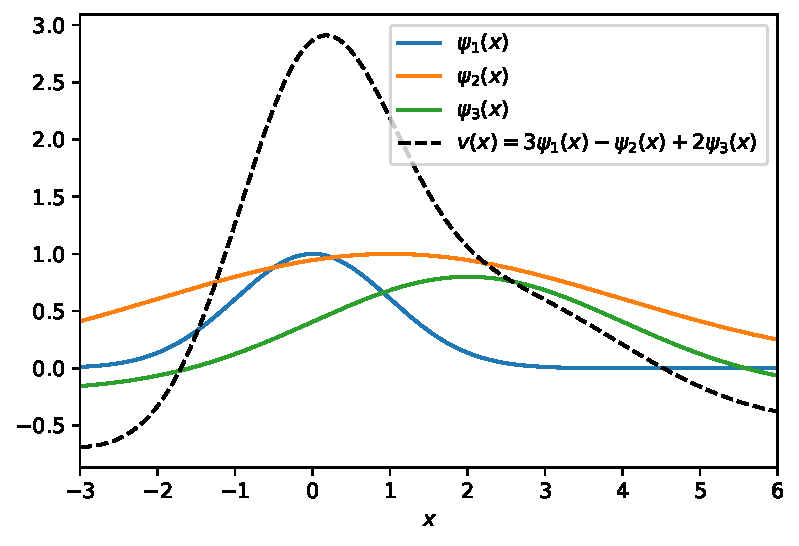
\includegraphics[width=\columnwidth]{figures/linear_parameterization.pdf}
\end{figure}
\end{columns}
\end{block}
Let's try again $v(0) = 0$:
\begin{itemize}
	\item
$\alpha^T \psi(0) = 0$ is a \textbf{linear equality constraint} in $\alpha$ (convex)
\end{itemize}
\end{frame}

\begin{frame}{Other ways we might want to constrain $v(x)$?}
\begin{block}{Nonnegativity constraints}
\begin{columns}
	\column{.6\textwidth}
For example, a Lyapunov function must be nonnegative
$$
v(x) = \alpha^T \psi(x) \geq 0 \text{ for all } x
$$
	\column{.35\textwidth}
\begin{figure}
	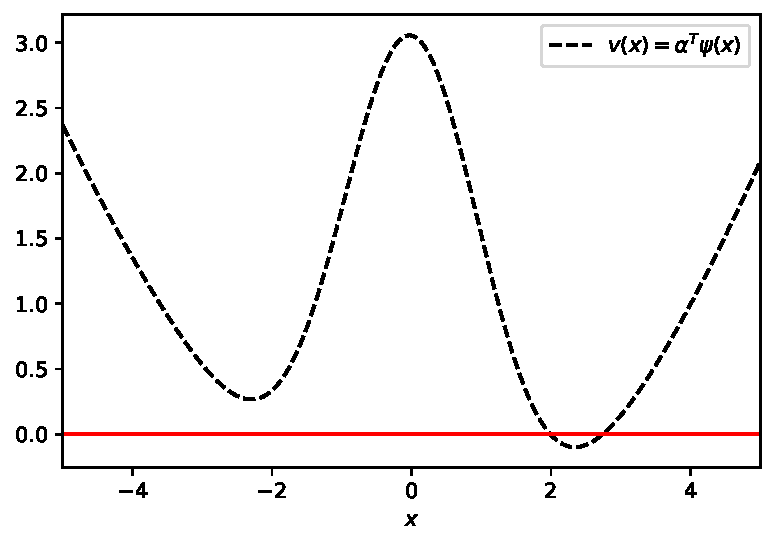
\includegraphics[width=\columnwidth]{figures/nonnegative.pdf}
\end{figure}
\end{columns}
\end{block}
Let's analyze the set
$$
\{ \alpha : \alpha^T \psi(x) \geq 0 \text{ for all } x\} \subseteq \mathbb R^r
$$
\end{frame}

\begin{frame}{Nonnegativity constraints and linear parameterizations}
\begin{block}{A seemingly positive observation}
The set $\{ \alpha : \alpha^T \psi(x) \geq 0\}$ is convex
\begin{itemize}
\item
Assume $v_1(x) = \alpha_1^T \psi(x) \geq 0$ and $v_2(x) = \alpha_2^T \psi(x) \geq 0$
\item
Then, for $\theta \in [0, 1]$,
$$
v(x) = [\theta \alpha_1 + (1 - \theta) \alpha_2]^T \psi(x) = \theta v_1(x)  + (1 - \theta) v_2(x)  \geq 0
$$
\end{itemize}
\end{block}
Is this enough to make the optimization over nonnegative $v(x)$ easy?
\begin{itemize}
\item
No, in general, no
\item
Except for a few cases, for a given $\alpha$, determining if $v(x) = \alpha^T \psi(x) \geq 0$ is NP-hard!
\item
We don't have a nice function to repel a point $\alpha$ from the boundary of the feasible set
\end{itemize}
\end{frame}

%\begin{frame}{A simple observation}
%%Constraining $\alpha$ so that $v(x) = \alpha^T \psi(x)$ is nonnegative seems pretty hard...
%\begin{block}{Sums-Of-Squares (SOS) decomposition}
%If we can find a matrix $Q \succeq 0$ and a vector of basis functions $m(x)$ such that
%$$
%v(x) = \alpha^T \psi(x) = m^T(x) Q m(x) \text{ for all } x
%$$
%then we certainly have $v(x) \geq 0$
%\end{block}
%There must be some sort of relation between the entries $\psi$ and $m$:
%\begin{itemize}
%\item
%Expanding the equality above we have
%$$
%\sum_{i=1}^r \alpha_i \psi_i(x) = \sum_{i,j=1}^q Q_{ij}m_i(x) m_j(x)
%$$
%\item
%Every entry of $\psi$ must be equal to the product of two elements of $m$
%\end{itemize}
%\end{frame}

\begin{frame}{Sums-of-squares parameterization}
%The linear parameterization $v(x) = \alpha^T \psi(x)$ can't handle nonnegativity constraints
What about a parameterization that is nonnegative by construction?
\begin{block}{Sums Of Squares (SOS)}
$$
v(x) = \psi^T(x) Q \psi(x) = \sum_{i,j=1}^r Q_{ij}\psi_i(x) \psi_j(x), \quad Q \succeq 0
$$
\begin{itemize}
\item
$Q$ is an $r$-by-$r$ matrix of coefficients (entries of $Q$ are our optimization variables)
\item
$\psi$ is an $r$-vector of basis functions
\end{itemize}
\end{block}
Remarks:
\begin{itemize}
\item
$v$ is still linear in $Q$ (e.g. $v(0) = 0$ is a \textbf{linear constraint} on the entries of $Q$)
\item
$Q \succeq 0$ is a \textbf{convex constraint}
\end{itemize}
\end{frame}

\begin{frame}{SOS constraints}
What if we want to certify that a given function $v(x)$ is nonnegative?
\begin{itemize}
\item
We can try to find a SOS decomposition $v(x) = \psi^T(x) Q \psi(x)$, with $Q \succeq 0$
\item
The issue however is how to pick $\psi(x)$...
\end{itemize}
\begin{block}{Example}
\begin{columns}
\column{.7\textwidth}
\begin{itemize}
\item
Consider $v(x) = \frac{1}{\sqrt{1 + x^2}}$
\item
This function is nonnegative for all $x$
\item
I don't quite know how to pick $\psi(x)$ here...
\end{itemize}
\column{.25\textwidth}
\begin{figure}
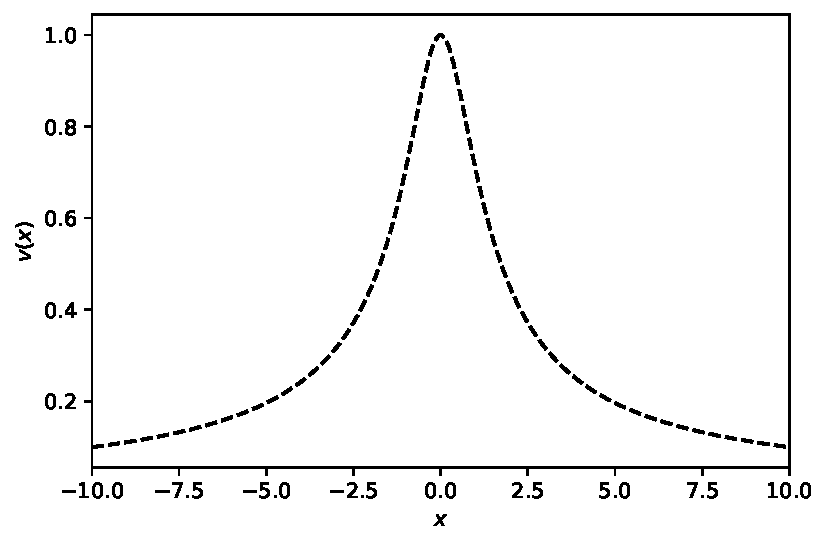
\includegraphics[width=\columnwidth]{figures/imq.pdf}
\end{figure}
\end{columns}
\end{block}
Can you think of any class of functions for which this approach might work?
\end{frame}

\begin{frame}{SOS polynomials}
With $v(x)$ polynomial of degree $2d$, we can just fill $\psi(x)$ with all the monomials up to degree $d$
\begin{block}{Example}
\begin{itemize}
\item
Given $v(x) = 2 - 2 x + 3 x^2 + 2 x^3 + x^4$, we set $\psi(x) = (1, x, x^2)$
\item
We look for $Q \succeq 0$ such that
$$
2 - 2 x + 3 x^2 + 2 x^3 + x^4 =
\begin{bmatrix} 1 \\ x \\ x^2 \end{bmatrix}^T
\begin{bmatrix} Q_{11} & Q_{12} & Q_{13} \\ Q_{12} & Q_{22} & Q_{23} \\ Q_{13} & Q_{23} & Q_{33} \end{bmatrix}
\begin{bmatrix} 1 \\ x \\ x^2 \end{bmatrix}
$$
\item
Comparing the coefficients we get \textbf{linear constraints} on $Q$, e.g., $Q_{11} = 2$
\end{itemize}
\end{block}
\begin{itemize}
\item
This works even if the coefficients of $v$ are (linear functions of) optimization variables!
\item
Other classes of functions could do the job, but polynomials have many other useful properties
\end{itemize}

\end{frame}

%\begin{frame}{Sums-of-squares polynomials}
%What about certifying that a polynomial $v(x)$ is nonnegative for all $x$?
%\begin{itemize}
%\item
%\end{itemize}
%Consider the scalar case $x \in R$ and show that with generic basis functions we can't ask $\frac{d v}{d x} (x) \geq 0$ for all $x$
%From here one we'll stick to polynomials but we could think of something different
%\end{frame}

%\begin{frame}{Sums-of-squares constraints}
%What if we want a given function $v(x)$ to be nonnegative?
%\begin{itemize}
%\item
%In Lyapunov analysis we require $\frac{\partial v}{\partial x} (x) f(x) \leq 0$ for all $x$
%\end{itemize}
%\end{frame}

%\begin{frame}{Sums-of-squares constraints}
%What if we want a linear functional of $v(x)$ to be nonnegative?
%\begin{itemize}
%\item
%In Lyapunov analysis we require $\frac{\partial v}{\partial x} (x) f(x) \leq 0$ for all $x$
%\end{itemize}
%\begin{block}{Example}
%\begin{itemize}
%\item
%Consider a polynomial $v(x) = \alpha_0 + \alpha_1 x + \alpha_2 x^2 + \alpha_3 x^3$
%\begin{itemize}
%\item
%Simple linear parameterization (not necessarily SOS)
%\item
%Basis functions $\phi_i(x)$ are monomials $x^i$
%\end{itemize}
%\item
%Say we want $\frac{d v}{d x} (x) \geq 0$ for all $x$
%\item
%For $Q \succeq 0$, we require
%\vspace{-3mm}
%$$
%\frac{d v}{d x} (x) = \alpha_1 + 2 \alpha_2 x + 3 \alpha_3 x^2 = \begin{bmatrix} 1 \\ x\end{bmatrix}^T Q \begin{bmatrix} 1 \\ x\end{bmatrix} = Q_{11} + 2 Q_{12} x + Q_{22} x^2
%$$
%\vspace{-4mm}
%\item
%These are just linear constraints: $\alpha_1 = Q_{11}$, $2 \alpha_2 = 2 Q_{12}$, $3 \alpha_3 = Q_{22}$
%\item
%Do you see what's special about polynomials here? 
%\end{itemize}
%\end{block}
%\end{frame}

\begin{frame}{The power of SOS optimization \href{https://colab.research.google.com/github/TobiaMarcucci/optimal_control_pisa/blob/master/demos/six_hump_camel.ipynb}{\beamergotobutton{Try this in Drake}}}
\begin{columns}
	\column{.7\textwidth}
\begin{itemize}
\item
Minimize the six-hump-camel function
$$
\min_x p(x) = 4 x_1^2 + x_1 x_2 - 4 x_2^2 - 2.1 x_1^4 + 4 x_2^4 + x_1^6 / 3
$$
\item
Write it as
\begin{align*}
\max_{ \lambda, Q} \ & \lambda \\
\text{subject to} \ &  p(x) - \lambda \text{ is SOS}
\end{align*}
\item
Where ``is SOS'' means ``equal to a SOS polynomial in $x$ parameterized by $Q$''
\end{itemize}
\column{.3\textwidth}
\vspace{-5mm}
\begin{figure}
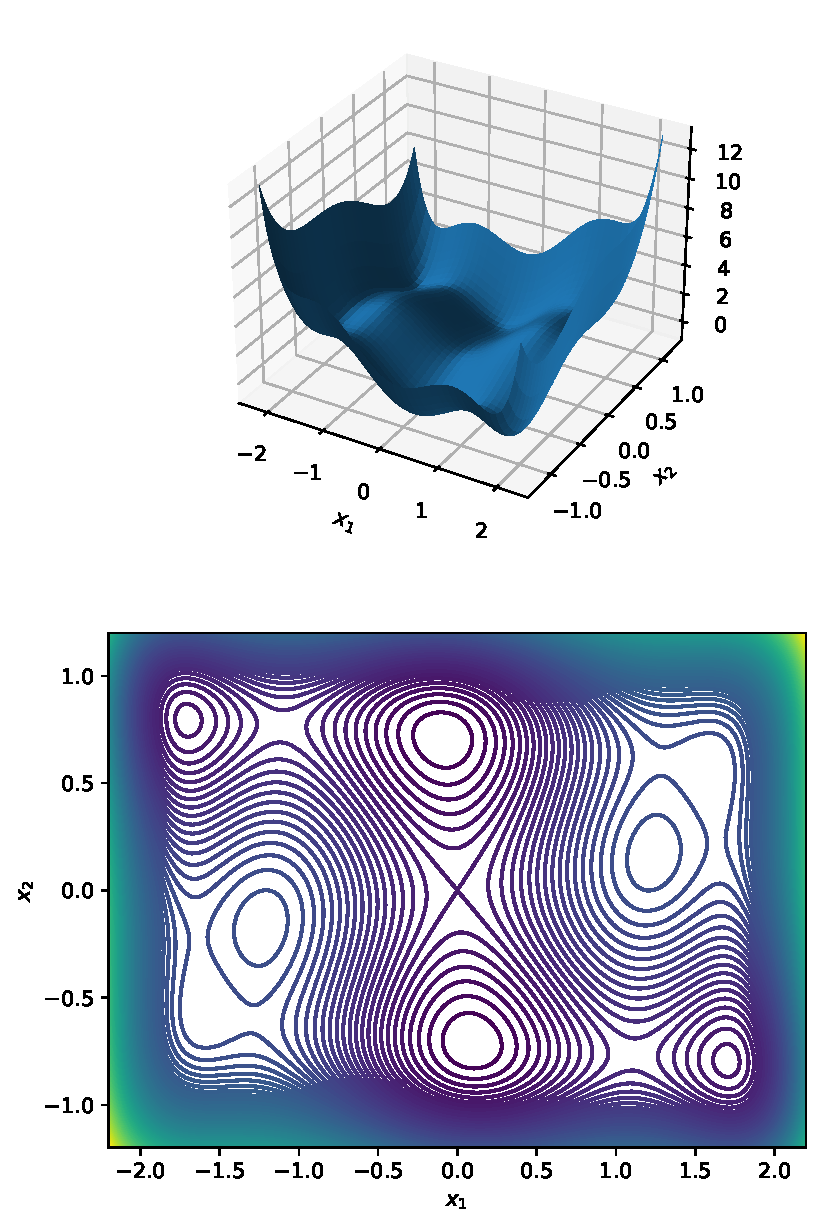
\includegraphics[width=\columnwidth]{figures/camel.pdf}
\end{figure}
\end{columns}
\end{frame}

\begin{frame}{Did we just solve global optimization over polynomials?}
\begin{columns}
\column{.6\textwidth}
Not all the nonnegative polynomials are SOS...
\begin{itemize}
\item
Hilbert in 1888\footnotemark showed that ``SOS = nonnegative'' only in 3 cases\footnotemark:
\begin{itemize}
\item
Univariate polynomials (1 variable)
\item
Quadratic polynomials (degree 2)
\item
Bivariate quartics (2 variables, degree 4)
\end{itemize}
\item
Famous counterexample by Motzkin
$$x_1^4 x_2^2 + x_1^2 x_2^4 + 1 - 3 x_1^2 x_2 ^2$$
\item
However, counterexamples are ``rare enough that people give names to them''
\end{itemize}
\column{.25\textwidth}
\begin{figure}
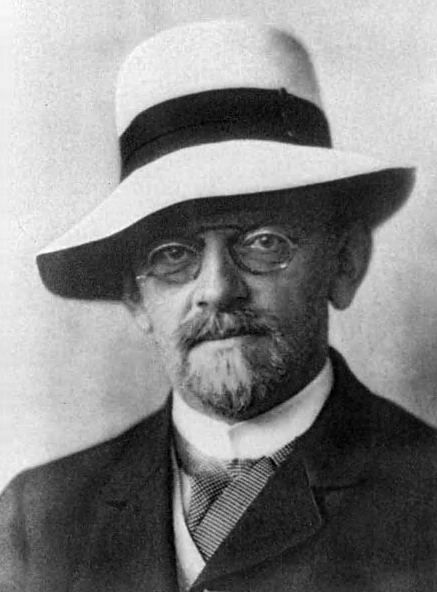
\includegraphics[width=.4\columnwidth]{figures/hilbert.jpg}
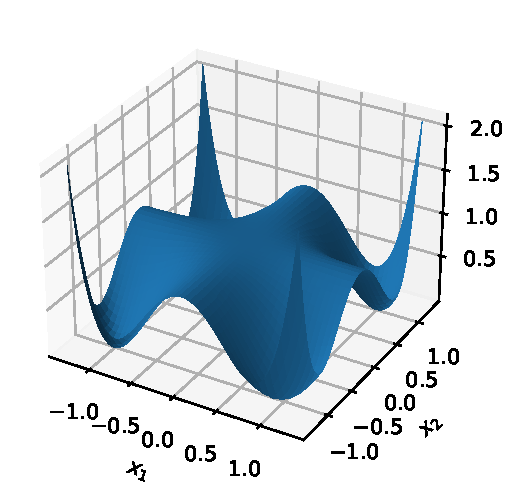
\includegraphics[width=\columnwidth]{figures/motzkin.pdf}
\end{figure}
\end{columns}
\footnotetext[1]{Hilbert - ``Ueber die Darstellung definiter Formen als Summe von Formenquadraten''}
\footnotetext[2]{See also \href{https://en.wikipedia.org/wiki/Hilbert\%27s_seventeenth_problem}{{\color{blue}Hilbert's 17th problem}}}
\end{frame}

\begin{frame}{One more trick: S-procedure}
\begin{itemize}
\item
To check if the polynomial $v(x)$ is nonnegative over the set
$$
\{ x :  g(x) = 0 \}
$$
with $g(x)$ polynomial, we can solve
$$
\text{find a polynomial } \lambda : v(x) + \lambda(x) g(x) \text{ is SOS}
$$
\item
Similarly, for the set
$$
\{ x :  g(x) \leq 0 \}
$$
we can solve
$$
\text{find a SOS polynomial } \lambda : v(x) + \lambda(x) g(x) \text{ is SOS}
$$
\end{itemize}
\end{frame}

\section{Design of Lyapunov functions}
\begin{frame}
\huge
\centering
{\color{darkred} Design of Lyapunov functions}
\end{frame}

\begin{frame}{Recap on Lyapunov stability}
\begin{columns}
\column{.5\textwidth}
The equilibrium $x=0$ for the system $\dot x = f(x)$ is:
\begin{itemize}
\item
\textbf{stable} if, for all $\varepsilon > 0$, there exists $\delta > 0$ such that
$$
\|x(0)\| < \delta \Rightarrow \|x(t)\| < \varepsilon \text{ for all }  t \geq 0
$$
\item
\textbf{asymptotically stable} if it is stable, and $\lim_{t \rightarrow \infty} \| x(t)\| = 0$
\end{itemize}
\column{.4\textwidth}
\begin{figure}
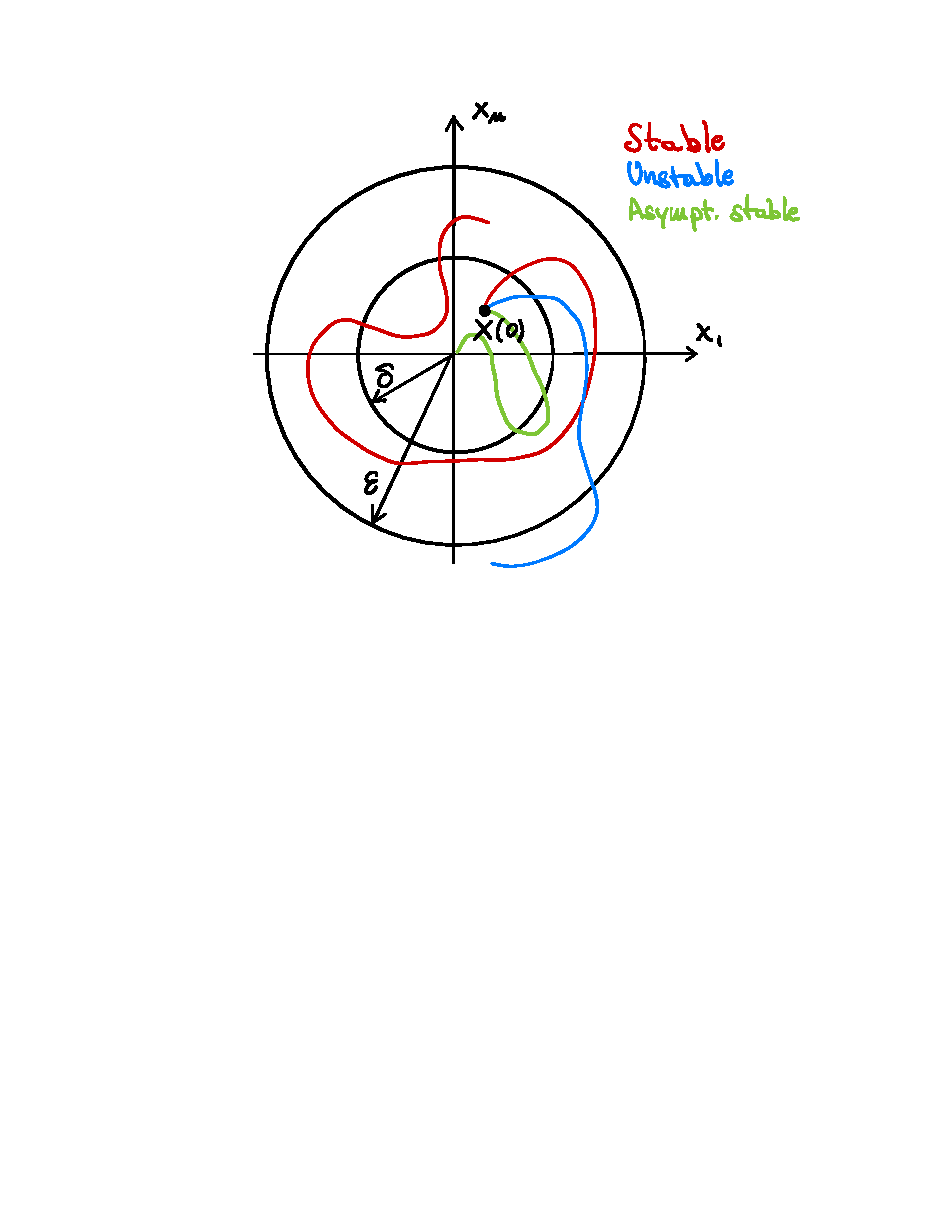
\includegraphics[width=\columnwidth]{figures/stability.pdf}
\end{figure}
\end{columns}
\end{frame}

\begin{frame}{Recap on Lyapunov direct method}
\begin{columns}
\column{.6\textwidth}
The equilibrium $x=0$ for the system $\dot x = f(x)$ is:
\begin{itemize}
\item
\textbf{stable} iff there exists $v(x)$ such that
$$
v(0) = 0, \quad v(x) > 0 \text{ for all } x \neq 0,
$$
and
$$
\dot v(x) = \frac{\partial v}{\partial x}(x) f(x) \leq 0 \text{ for all }  x \neq 0
$$
\item
\textbf{asymptotically stable} iff
$$
\dot v(x) < 0 \text{ for all }  x \neq 0
$$
\end{itemize}
\column{.4\textwidth}
\begin{figure}
	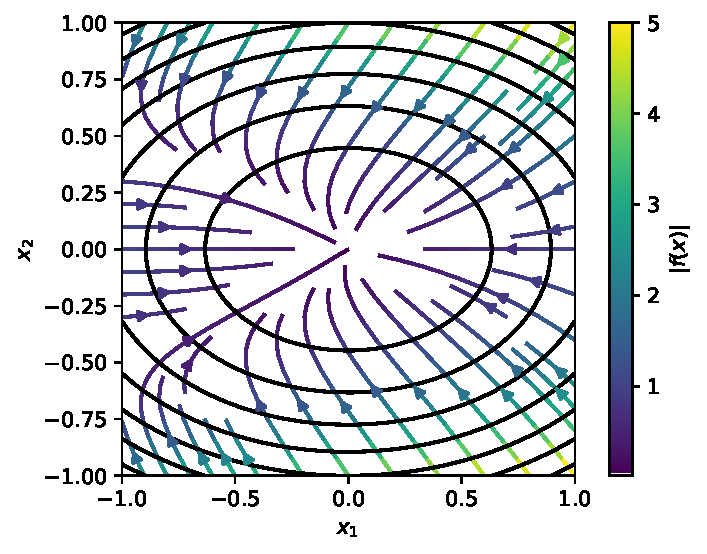
\includegraphics[width=\columnwidth]{figures/lyapunov_poly.pdf}
\end{figure}
\end{columns}
\end{frame}


\begin{frame}{Design of Lyapunov functions via SOS}
SOS parameterization of the Lyapunov function
$$
v(x) = \psi^T(x) Q \psi(x), \quad Q \succeq 0
$$
Filling $\psi(x)$ with monomials is the natural choice:
\begin{itemize}
\item
It works in the linear case $f(x) = A x$ (we always have $v(x) = x^T P x$)
\item
If $f(x)$ is polynomial, then
$$
\dot v(x) = \frac{\partial v}{\partial x}(x) f(x)
$$
is also polynomial, and its coefficients are linear in $Q$
\item
If $f(x)$ is not polynomial we can use, e.g., Taylor approximation
\end{itemize}
\end{frame}

\begin{frame}{Design of Lyapunov functions via SOS
\href{https://colab.research.google.com/github/TobiaMarcucci/optimal_control_pisa/blob/master/demos/lyapunov_poly.ipynb}{\beamergotobutton{Try this in Drake}}}
\begin{block}{The overall SOS program}
$$
\text{find } v(x) \text{ SOS} : \frac{\partial v}{\partial x}(x) f(x) \text{ is SOS}
$$
\end{block}
Miscellaneous observations:
\begin{itemize}
\item
To avoid the trivial solution $v(x) = 0$ we can add a linear constraint like $v(1) = 1$
\item
Be aware: not all the stable polynomial systems admit a polynomial Lyapunov function\footnote{Ahmadi, Krstic, Parrilo - ``A Globally Asymptotically Stable Polynomial Vector Field with no Polynomial Lyapunov Function''}
\end{itemize}
\end{frame}

\begin{frame}{Verification of nonpolynomial systems via SOS
\href{https://colab.research.google.com/github/TobiaMarcucci/optimal_control_pisa/blob/master/demos/lyapunov_pendulum.ipynb}{\beamergotobutton{Try this in Drake}}}
\begin{columns}
\column{.65\textwidth}
\begin{itemize}
\item
Some non-polynomial systems can be verified exactly using SOS\footnotemark
$$
\dot x_1 = x_2, \quad
\dot x_2 = - x_2 - \sin(x_1)
$$
\item
Introduce auxiliary variables $s = \sin(x_1)$, $c = \cos(x_1)$
\item
Substitute to get the polynomial system
$$
\dot s = c x_2, \quad
\dot c = - s x_2, \quad
\dot x_2 = - x_2 - s
$$
subject to the polynomial constraint $s^2 + c^2 = 1$
\end{itemize}
\column{.3\textwidth}
\begin{figure}[h]
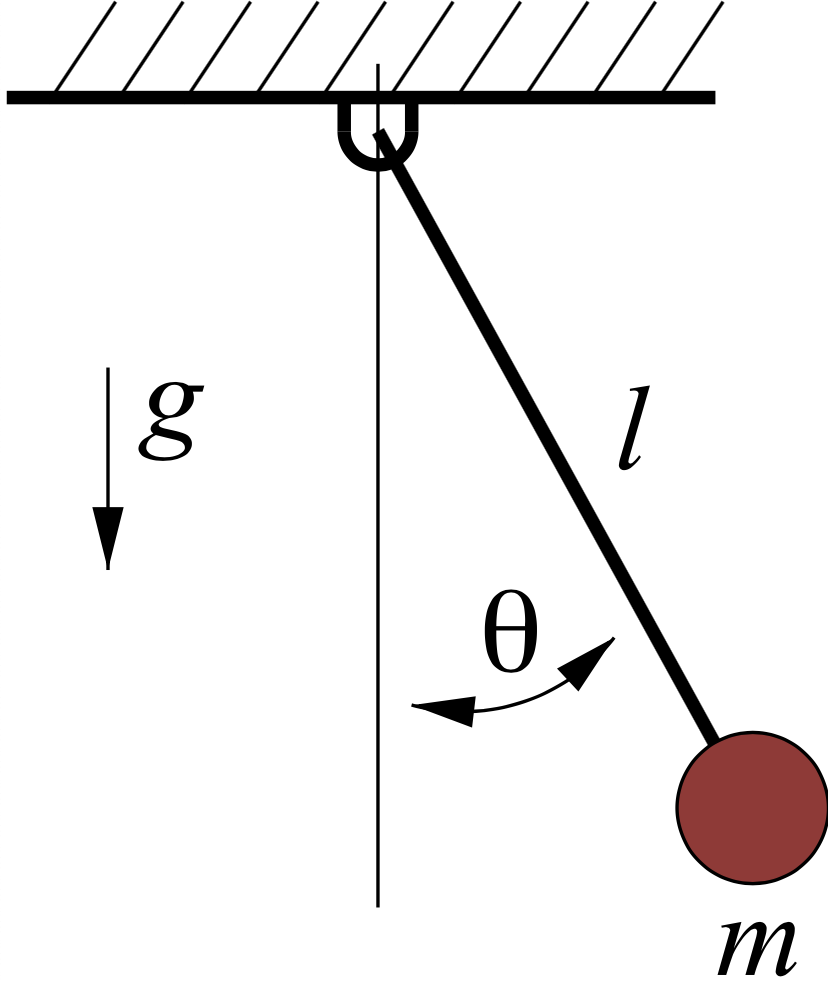
\includegraphics[width=.3\columnwidth]{figures/simple_pend.png}
\end{figure}
\begin{figure}[h]
	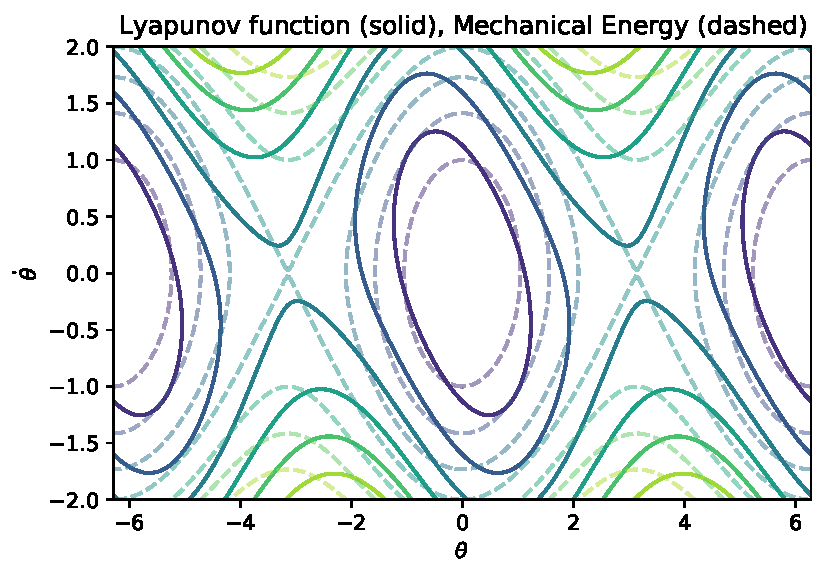
\includegraphics[width=\columnwidth]{figures/lyapunov_pendulum.pdf}
\end{figure}
\end{columns}
\footnotetext[1]{See also Papachristodoulou, Prajna - ``Analysis of Non-polynomial Systems using the Sum of Squares Decomposition''}
\end{frame}

\begin{frame}{Bonus: approximation of region of attraction}
Time-reversed Van der Pol oscillator
\begin{align*}
\dot x_1 &= - x_2 \\
\dot x_2 &= x_1 + (x_1^2 - 1) x_2
\end{align*}
\begin{columns}
\column{.5\textwidth}
Maximize volume of level set
\begin{figure}[h]
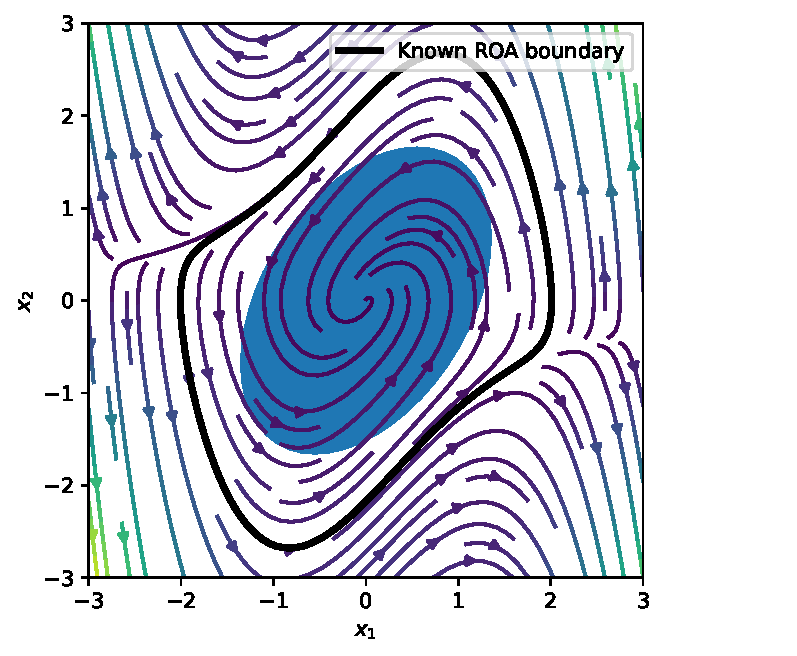
\includegraphics[width=.5\columnwidth]{figures/van_der_pol_roa_quadratic.pdf}
\end{figure}
\column{.5\textwidth}
Alternate between maximization of level set and reshape Lyapunov function
\begin{figure}[h]
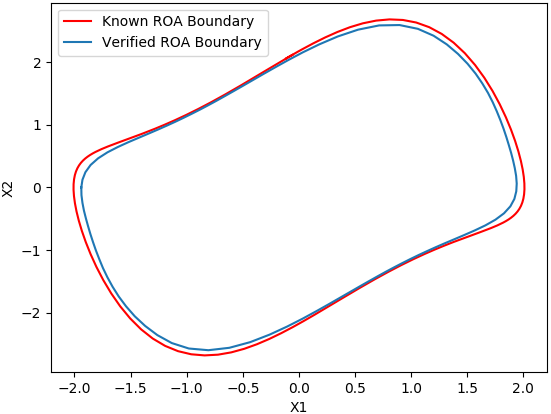
\includegraphics[width=.55\columnwidth]{figures/van_der_pol_roa.png}
\end{figure}
\end{columns}
\end{frame}

\begin{frame}{Control-Lypaunov function}
Can use use SOS + Lyapunov verification to design controllers? Unfortunately no...
\begin{itemize}
\item
We let $v(x)$ be a SOS polynomial
\item
We use a linear parameterization for $u(x)$ (polynomial)
\item
For simplicity, let the system be polynomial and control-affine
$$
\dot x = f(x) + G(x) u
$$
\item
Lyapunov condition becomes
$$
- \frac{\partial v}{\partial x}(x) [f(x) + G(x) u(x)] \text{ is SOS}
$$
\item
Multiplication of $\frac{\partial v}{\partial x}$ and $u$ leads to \textbf{nonlinear equality constraints}
\end{itemize}
\end{frame}

\section{Approximate dynamic programming}
\begin{frame}
\huge
\centering
{\color{darkred} Approximate dynamic programming}
\end{frame}

\begin{frame}{Hamilton-Jacobi-Bellman (HJB) equation}
How to arrive to the HJB equation
\begin{align*}
\min_{u \in U} \left\{ l(x, u) + \frac{\partial v}{\partial x} (x) f(x, u) \right\} = 0, \quad \text{for all } x
\end{align*}
from the Optimal Control Problem (OCP)
\begin{align*}
v(x_0) := \min_{u, x} \ &\int_0^\infty l(x(t), u(t)) dt \\
\text{subject to} \ & x(0) = x_0 \\
& \dot x(t) = f(x(t), u(t)), &&  \text{for all }t \in [0, \infty) \\
& u(t) \in U, &&  \text{for all }t \in [0, \infty)
\end{align*}
\end{frame}

\begin{frame}{HJB: informal derivation}
First order approximation of the control problem with time step $h$:
\begin{itemize}
\item
Cost function
$$
\int_0^\infty l(x(t), u(t)) dt
\approx
h \sum_{t=0}^\infty l(x_t, u_t)
$$
\item
Dynamics
$$
\dot x(t) = f(x(t), u(t))
\Rightarrow
x_{t+1} = x_t + h f(x_t, u_t)
$$
\item
Overall
\begin{align*}
v(x_0) := \min_{u, x} \ &h \sum_{t=0}^\infty l(x_t, u_t) \\
\text{subject to} \ & x_0 \text{ given} \\
& x_{t+1} = x_t + h f(x_t, u_t), &&  t = 0, \ldots, \infty \\
& u_t \in U, &&  t = 0, \ldots, \infty
\end{align*}
\end{itemize}
\end{frame}

\begin{frame}{HJB: informal derivation}
\begin{columns}
\column{.7\textwidth}
The dynamic-programming principle:
\begin{itemize}
\item
Assume $\mathbf x_0 = (x_0, x_1, x_2, x_3, \ldots)$ is the optimal trajectory from $x_0$ to the origin
\item
Because of the infinite horizon, the optimal trajectory $\mathbf x_1$ from $x_1$ to the origin must be
$(x_1, x_2, x_3, \ldots)$
\begin{itemize}
\item
Otherwise $(x_0, \mathbf x_1)$ would be better than $\mathbf x_0$ (contradiction)
\end{itemize}
\item
If we were to know the cost-to-go $v(x_1)$ from $x_1$, then we could just solve a one-step problem
\begin{align*}
v(x_0) & = \min_{u_0 \in U} \{ h l(x_0, u_0) + v(x_1) \} \\
& = \min_{u_0 \in U} \{ h l(x_0, u_0) + v(x_0 + h f(x_0, u_0)) \} \\
\end{align*}
\end{itemize}
\column{.3\textwidth}
\vspace{-5mm}
\begin{figure}
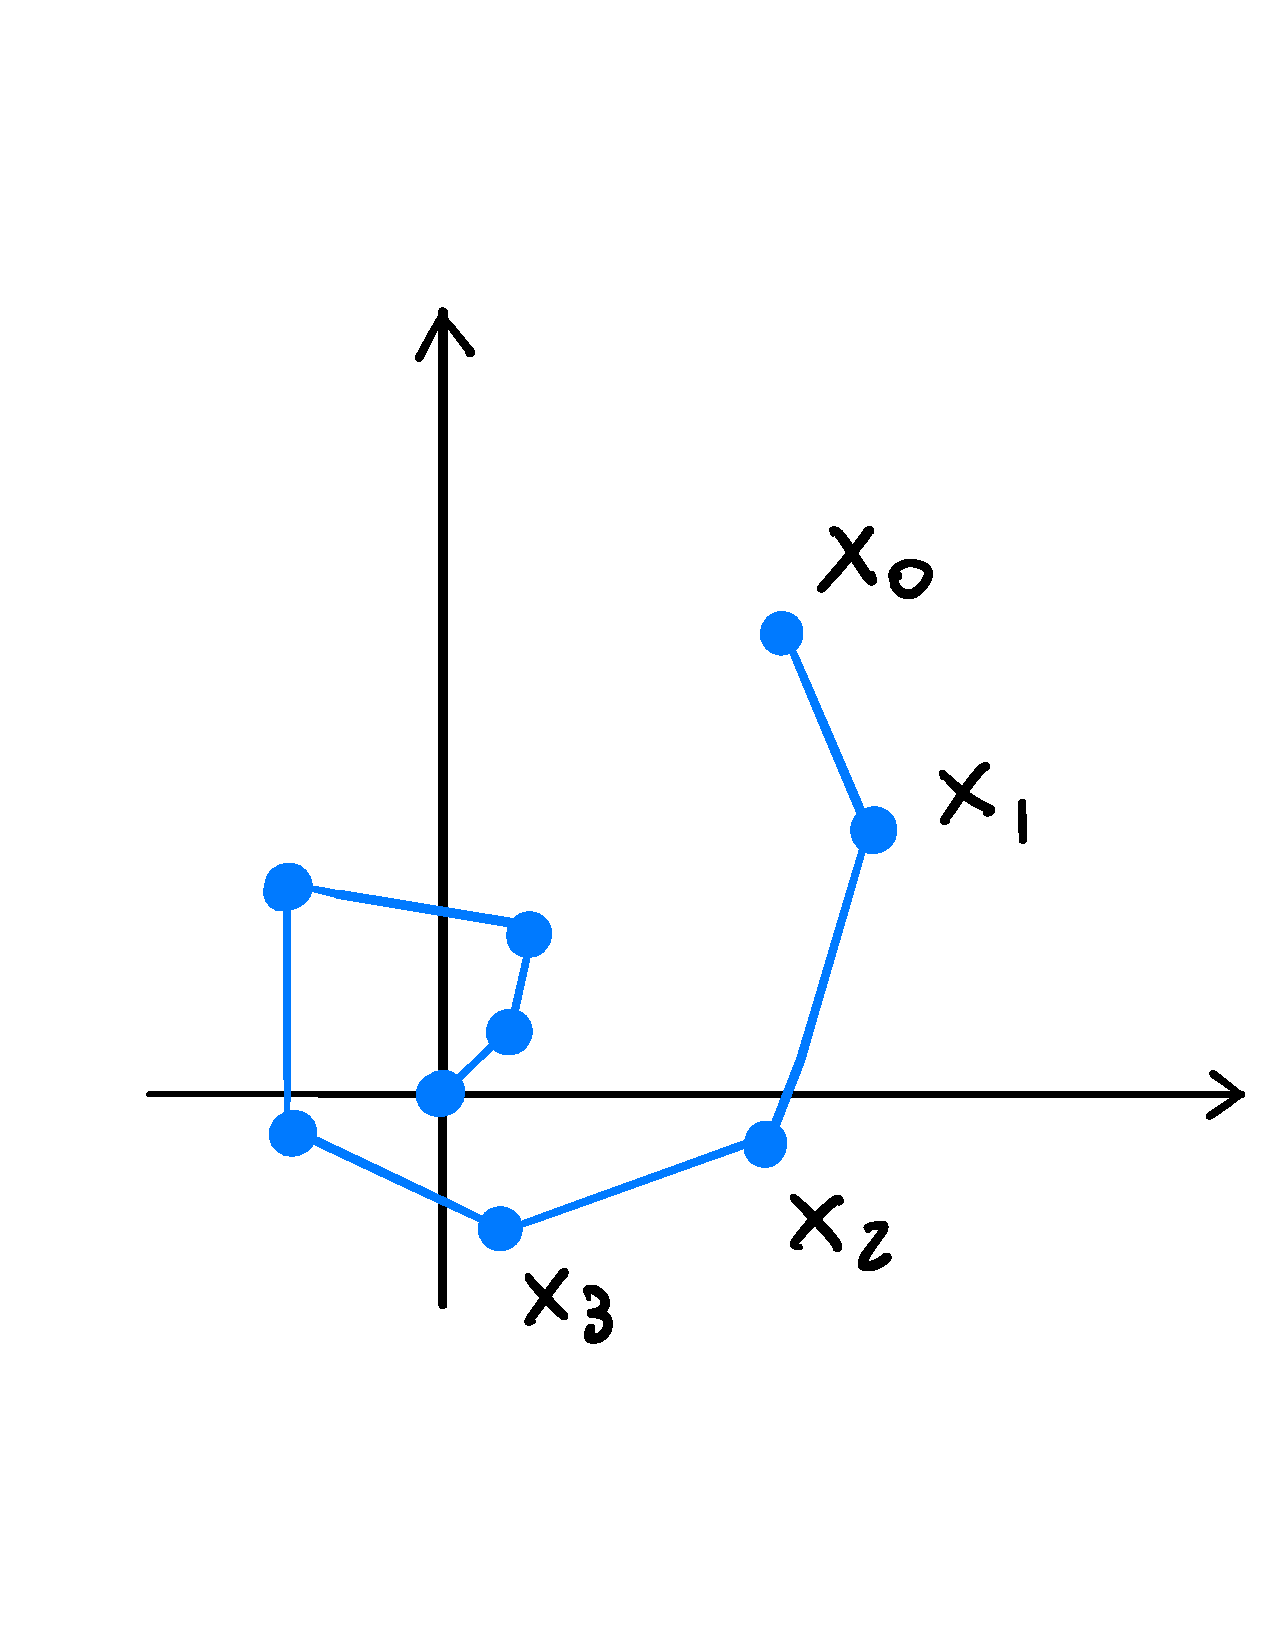
\includegraphics[width=\columnwidth]{figures/dp_principle.pdf}
\end{figure}
\end{columns}
\end{frame}

\begin{frame}{HJB: informal derivation}
\begin{itemize}
\item
If $h$ is very small
$$
v(x_0 + h f(x_0, u_0)) \approx v(x_0) + h \frac{\partial v}{\partial x} (x_0) f(x_0, u_0)
$$
\item
Substituting
$$
v(x_0) = \min_{u_0 \in U} \left\{ h l(x_0, u_0) +  v(x_0) + h \frac{\partial v}{\partial x} (x_0) f(x_0, u_0) \right\}
$$
\item
Simplifying $v(x_0)$ and dividing by $h$
$$
0 = \min_{u_0 \in U} \left\{ l(x_0, u_0) + \frac{\partial v}{\partial x} (x_0) f(x_0, u_0) \right\}
$$
\end{itemize}
Why ``informal''? Where does this derivation leak? (Think at the bang bang controller)
\end{frame}

\begin{frame}{Solving the HJB}
The HJB equation is a nonnlinear Partial Differential Equation (PDE)
\begin{itemize}
\item
Analytic solutions only in a few special cases (LQR)
\item
``Exact'' numerical solution is very hard (discretization of the state and control space)
\item
Can we still find approximate solutions that are ``good enough''?
\end{itemize}

\begin{block}{``One side of the HJB equation is convex''}
$$
\min_{u \in U} \left\{ l(x, u) + \frac{\partial v}{\partial x} (x) f(x, u) \right\} \geq 0, \quad \text{for all } x
$$
is equivalent to the \textbf{Bellman inequality}
$$
l(x, u) + \frac{\partial v}{\partial x} (x) f(x, u) \geq 0, \quad \text{for all } x \text{ and } u \in U
$$
\vspace{-5mm}
\begin{itemize}
\item
We can relax this condition via SOS!
\end{itemize}
\end{block}
\end{frame}

\begin{frame}{Bellman inequality}
What do we loose by enforcing only one side of the HJB equations?
\begin{itemize}
\item
Let $x(t)$ and $u(t)$ be the optimal trajectory and control from $x(0)$
\item
Integrate the Bellman inequality along the optimal trajectory
\begin{align*}
0 & \leq \int_0^\infty \left[ l(x(t), u(t)) + \frac{\partial v}{\partial x} (x(t)) f(x(t), u(t)) \right] dt \\
& = \int_0^\infty l(x(t), u(t)) dt + \int_0^\infty \dot v(x(t)) dt \\
& = \int_0^\infty l(x(t), u(t)) dt + v(x(\infty)) - v(x(0))
\end{align*}
\item
Let $v(0) = 0$, then $v(x)$ lower bounds the optimal value function
$$
v(x(0)) \leq \int_0^\infty l(x(t), u(t)) dt
$$
\end{itemize}
\end{frame}

\begin{frame}{SOS for approximate dynamic programming}
\begin{align*}
\max_v \ &\int_X v(x) dx \\
\text{subject to} \ & l(x, u) + \frac{\partial v}{\partial x} (x) f(x, u) \text{ is SOS for all } x \text{ and } u \in U \\
& v(0) = 0
\end{align*}
Interpretation:
\begin{itemize}
\item
Constraints ensure that $v(x)$ lower bounds the value function
\item
Objective ``pushes up'' $v(x)$ over the set $X$
\item
As the degree of $v(x)$ increases, we get a better and better approximation of the value function over $X$
\end{itemize}
\end{frame}

\begin{frame}{Toy approximate-DP problem}
\begin{itemize}
\item
Scalar dynamics
\end{itemize}
\end{frame}

\begin{frame}{Recover the optimal controller}

\end{frame}

\begin{frame}{Pendulum swing up}
	
\end{frame}

\section{Bibliography}
\begin{frame}{Bibliography}
\footnotesize
Convex optimization:
\begin{itemize}
\item
Boyd, Vandenberghe - ``Convex Optimization''
\end{itemize}
Semidefinite programming:
\begin{itemize}
\item
Vandenberghe, Boyd - ``Semidefinite programming''
\item
Boyd, Vandenberghe - ``Convex Optimization''
\end{itemize}
Sums-of-Squares optimization:
\begin{itemize}
\item
Parrilo - ``Structured semidefinite programs and semialgebraic geometry methods in robustness and optimization''
\item
Blekherman, Parrilo, Thomas - ``Semidefinite Optimization and Convex Algebraic Geometry''
\end{itemize}
Lyapunov stability:
\begin{itemize}
\item
Khalil - ``Nonlinear Systems''
\end{itemize}
\end{frame}

\begin{frame}{Bibliography}
\footnotesize
Dynamic programming:
\begin{itemize}
\item
Bertsekas - ``Dynamic Programming and Optimal Control''
\item
Kirk - ``Optimal Control Theory an Introduction''
\item
Bressan, Piccoli - ``Introduction to the Mathematical Theory of Control''
\end{itemize}
Hamilton-Jacobi-Bellman equation:
\begin{itemize}
\item
Evans - ``Partial Differential Equations''
\end{itemize}
Approximate dynamic programming:
\begin{itemize}
\item
\end{itemize}
Software:
\begin{itemize}
\item
\href{https://drake.mit.edu}{{\color{blue}Drake}}
\end{itemize}
\end{frame}

\end{document}